\documentclass[12pt]{book}
\usepackage[utf8]{inputenc}
\usepackage{hyperref}
\usepackage{graphicx}

\title{Petit guide d'utilisation de Linux Mint}
\author{Association Eisenia}
\date{2021}

\begin{document}
\maketitle

\newpage
\renewcommand{\contentsname}{Table des matières}
\tableofcontents

\renewcommand{\chaptername}{Chapitre}
\chapter{Introduction}
	\section{Introduction générale}
	\section{Introduction au logiciel libre}

\chapter{Environnement Linux Mint}
\section{Se familiariser avec l'environnement Linux Mint}
	\subsection{Le bureau}
	\subsection{La barre des tâches}
		La barre des tâches se situe en bas de l'écran.
		Le bouton tout à gauche permet d'ouvrir le "menu démarrer" (voir section \ref{sec:menudemarrer}). 
	\subsection{Le menu démarrer}\label{sec:menudemarrer}
		Le menu démarrer se décompose en quatre parties :
		\begin{itemize}
			\item La barre latérale tout à gauche contient lesz outils de bases : le Navigateur Firefox (voir Sections \ref{sec:descfirefox} et \ref{sec:utiliserfirefox}); l'invit de commande (voir Section \ref{sec:utiliserterminal}); ...
			\item Le menu principal au centre contient toutes les catégories de logiciel
			\item Le menu de droite contient les éléments contenu dans la catégorie sélectionnée
			\item La barre de recherche en haut permet de rechercher par mots-clés 
		\end{itemize}
	\subsection{Le gestionnaire de fichiers}
		Le gestionnaire de fichier se trouve sur la barre des tâches, c'est l'icône qui est représenté par un petit dossier vert.\newline
		
	\subsection{Eteindre l'ordinateur}
		Lorsque vous avez terminer votre utilisation, il faut éteindre l'ordinateur; L'éteindre après chaque utilisation est important. Cela permet notamment de réduire la chaleur des composants, de résoudre certains bugs liés à une trop longue utilisation, etc.\newline
		Pour cela, ouvrez le menu démarrer et cliquez sur l'icône rouge en bas à gauche de la barre latérale.
		Une boîte de dialogue s'ouvre et vous propose plusieurs options.
		Cliquez sur celle toute à droite "Eteindre".
		Vorte ordinateur affiche le logo de Linux Mint puis s'éteint.

\section{Utiliser un périphérique amovible}

\section{Paramètrer le compte}
	Dans cette section, nous allons voir comment nous pouvons personnalier l'ordinateur.
	Changer le nom d'utilisateur, le mot de passe, l'avatar... peut être bien utile et plus agréable.\newline
	\subsection{Modifier le nom de l'utilisateur}
	\subsection{Modifier le mot de passe}
	\subsection{Modifier l'avatar}

\chapter{Logiciels}
Dans ce chapitre, nous allons aborder quelques logiciels libres de base pour bien démarrer avec son ordinateur.
Nous présenterons tout d'abord le pack LibreOffice permettant d'éditer une multitude de documents différents.
Puis nous présentenrons le navigateur web Firefox de Mozila.
Enfin, nous présenterons le lecteur multimédia VLC.
La liste de logiciels libres que nous vous proposons ici est non-exhaustive.
Il existe beaucoup d'autres logiciels très pratique selon vos besoins.\
C'est pour quoi, nous expliquons dans la dernière section de ce chapitre comment installer de nouveaux logiciels sur votre ordinateurs.
\section{Les logiciels indispensables pour bien démarrer}
	\subsection{Le pack LibreOffice}
		Le pack LibreOffice est indispensable lorsque l'on souhaite rédiger des documents de toute sorte.\newline
		Il est composé de plusieurs lorgiciels.
		\begin{itemize}
			\item LibreOffice writer vous permet de rédiger des documents textes et de les mettre en forme.
			Ces documents sont au format .odt. 
			Il est aussi possible d'imprimer ses documents ou de les exporter au format .pdf via LibreOffice Writer.
			\item LibreOffice Calc vous permet de créer et d'utiliser des classeurs.
			Ces documents sont au format .ods. 
			Ils sont très utilisés pour faire des feuilles de calculs, enregistrer des données, etc.
			\item LibreOffice Impress vous permet de créer des diaporamas. 
			Ces documents sont au format .odp.
			LibreOffice Impress vous sera très utile pour préparer des supports visuels, des diaporamas pour des exposés, des réunions, etc.
			Il vous sera possible d'exporter votre document au format .pdf.
			\item LibreOffice Draw vous permet de faire toute sorte de dessins.
			Ces documents sont au format .odg.
			Très pratique pour faire un petit dessin rapide, un schéma plus complexe ou bien encore un support visuel.
			\item LibreOffice Math vous permet de rédiger des formules mathématiques.
			Ces documents sont au format .odf;
			Cet outil vous permet de prnedre en notes des formules mathématiquesdiverses, d'utiliser des opérateurs (unitaires, binaires, logiques...), des relations, de rédiger des matrices, d'utiliser des symboles, etc.
			\item LibreOffice Base vous permet de créer et de gérer une base de données relationnelles.
			Il est possible de créer une nouvelle base ou bien de se connecter à une base (JDBC par exemple). 
		\end{itemize}
	\subsection{Mozila Firefox}\label{sec:descfirefox}
		Le navigateur Mozila Firefox va vous permettre d'afficher des pages web.\newline
		Ce navigateur très connu et utilisé vous offre beacoup de paramètres d'affichage, de langue mais aussi de sécurité.\par
		Mozila Firefox est un navigateur libre.
		C'est-à-dire qu'il n'appartient pas à une entreprise dont le but est de faire de l'argent avec ce logiciel.
		Pour un navigateur web, cela garanti notamment une certaine sécurité sur nos données personnelles.
		En effet, Firefox n'a aucun intérêt à revendre les données de ces utilisateurs, donc il en collecte que très peu.\par
		Ce navigateur permet également de bloquer les traqueurs publicitaires.
		...
	\subsection{VLC}

\section{Installer de nouveaux logiciels}
	\textit{Ici, description de l'outil logithèque.}

\chapter{Internet}
Maintenant que nous nous sommes familiarisés avec cet environnement, il est temps d'aller surfer sur le web.\newline
Dans ce chapitre, nous allons voir dans un premier temps comment nous connecter à internet.
Dans un deuxième temps, nous allons mieux étudier le navigateur Mozila Firefox qui sera notre "porte" pour aller sur internet.
Et dans un troisième temps, nous allons voir comment utiliser le moteur de recherche Lilo qui nous permettra de faires nos premières recherches sur internet.
\section{Se connecter à son réseau}
	Avant toute chose, nous devons être connecter à Internet. C'est-à-dire que nous devons établir un lien entre l'ordinateur et le réseau.
	Pour cela, il y a deux façons de procéder :
	\begin{enumerate}
		\item en se connectant via un un câble reliant l'ordinateur à la box ;
		\item en se connectant via un le WiFi.
	\end{enumerate}
	\subsection{Avec un câble éthernet}
		Avec votre ordinateur, un câble RJ45 (éthernet) vous a été fourni.
		L'embout ressemble à ceci :
		\begin{figure}[h]
			\centering
			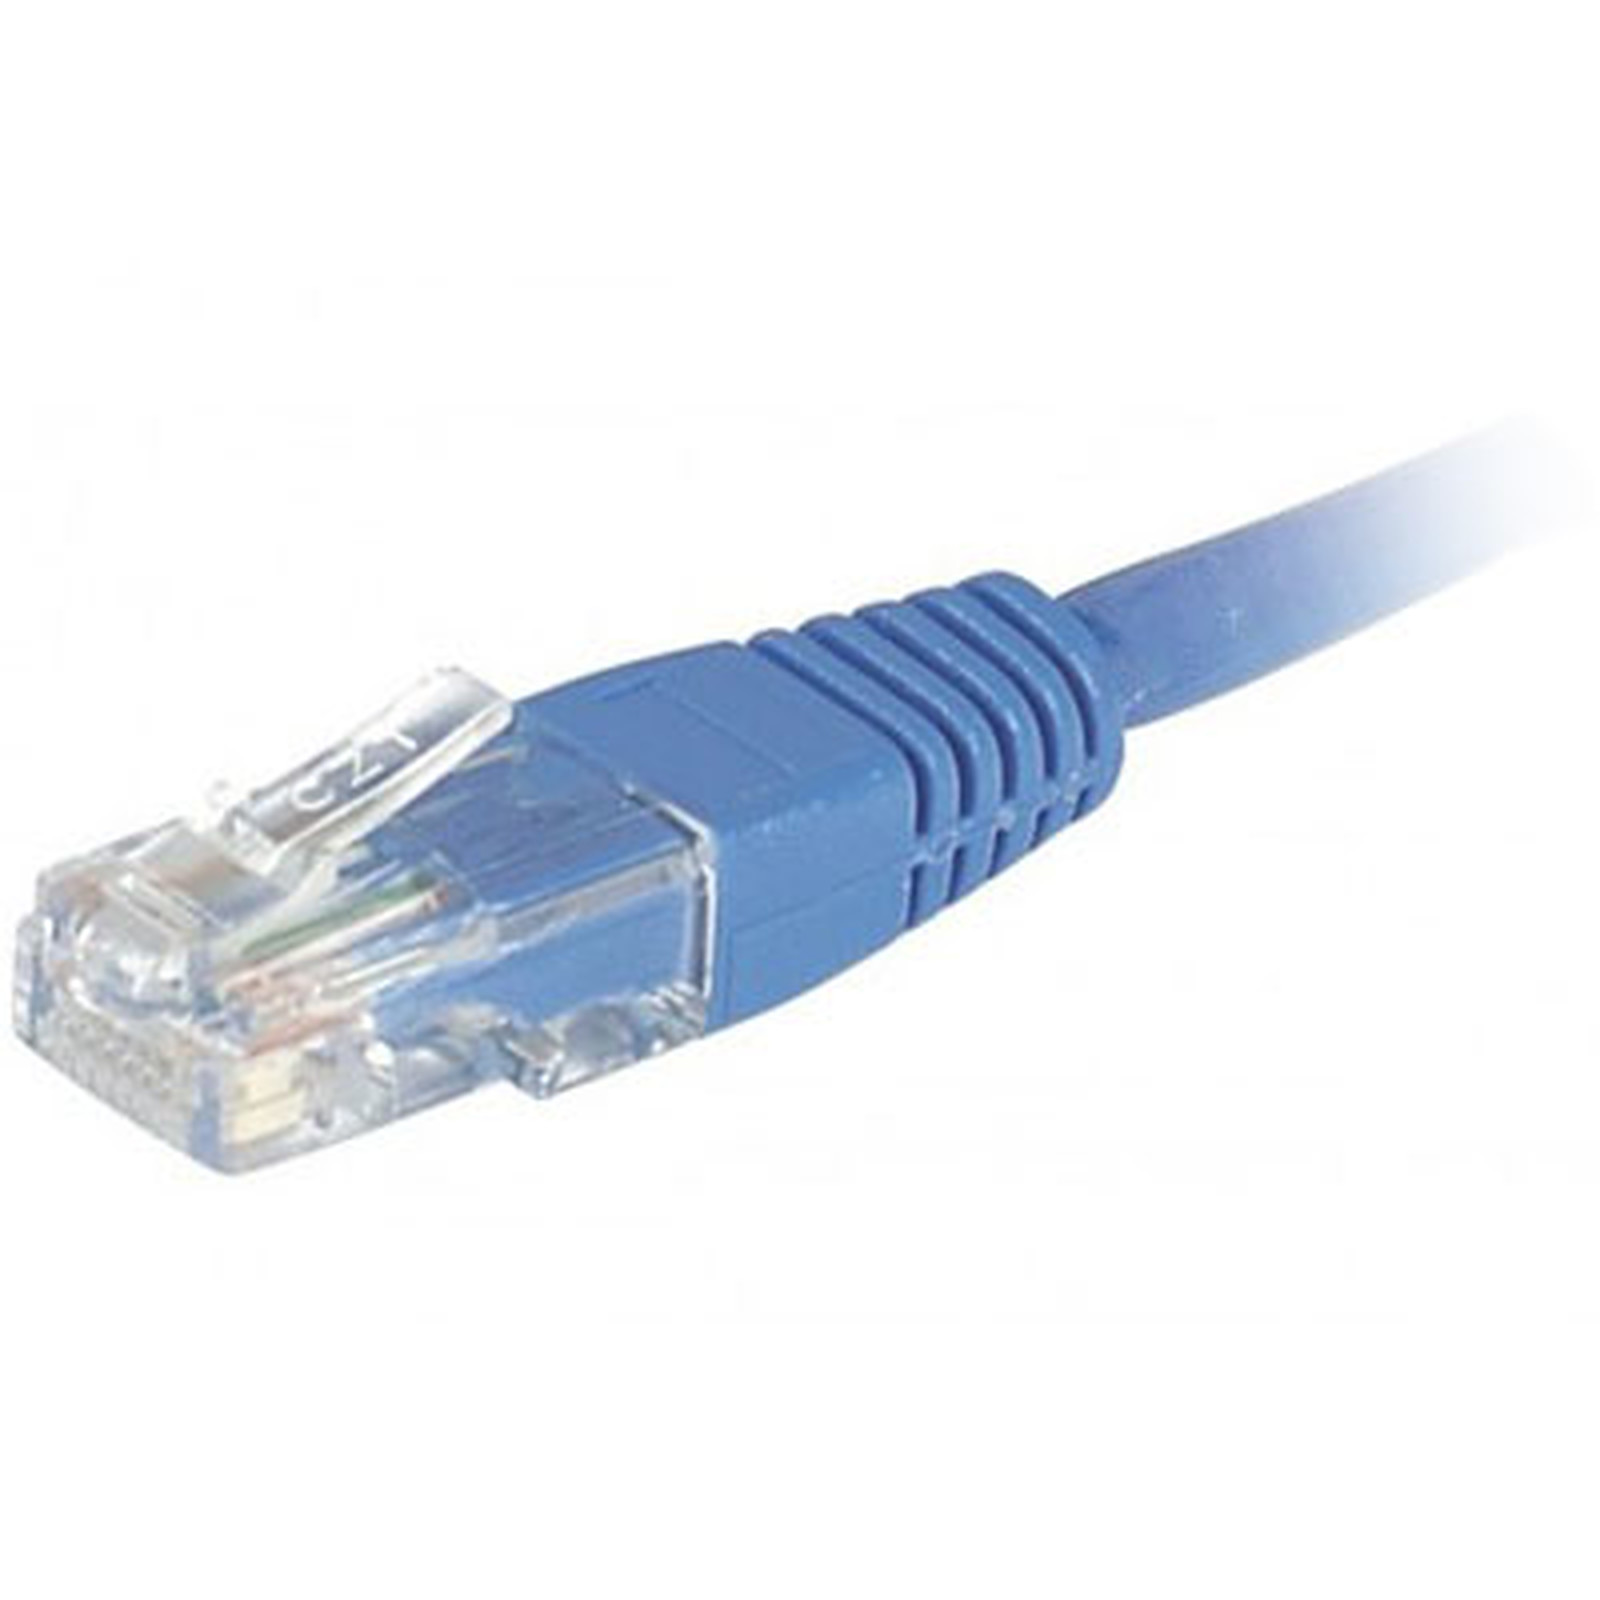
\includegraphics[scale=0.05]{include/rj45.jpg}
			\label{fig:rj45}
			\caption{Câble éthernet RJ45}
		\end{figure}\newline
		Ce câble se branche d'un côté à votre ordinateur et de l'autre à votre box (ou dans la prise éthernet de votre mur si elle existe).\par
		Une fois branché des deux côtés, l'icône "Internet" à droite sur la barre des tâches doit avoir changé et ressembler à ceci :
%		\begin{figure}
%			\centering
%			\label{fig:iconeconnecte}
%			\caption{Icône Internet "connecté"}
%		\end{figure}
		\newline
		Une notification a pu aussi apparaître tout en haut à droite de votre écran.
		Elle doit ressember à ceci :
%		\begin{figure}
%			\centering
%			\label{fig:notifconnecte}
%			\caption{Notification "ordinateur connecté" à Internet}
%		\end{figure}
		Une fois que cette icône est apparue, félicitations, vous êtes connecté à Internet !
	\subsection{Avec le WiFi}
		Avant de commencer.
		Si vous disposez d'un ordinateur portable, votre ordinateur dispose d'un système de connexion au WiFi intégré et vous pouvez directement essayer de vous connecter.
		Si vous disposez d'un ordinateur fixe, vous aurez probablement besoin d'un dispositif de connexion WiFi externe.
		Nous vous conseillons d'utiliser une clé USB WiFi.
		Elles sont très simple d'utilisation.
		Pour certaines, il suffit de les brancher dans l'ordinateur et vous pourrez vous connecter aux réseaux WiFi.\par
		Pour vous connecter, cliquez sur l'icône "Connexion à Internet" à droite sur la barre des tâches.
		Un petit menu s'affiche alors.
		Cliquez sur le réseau WiFi qui vous intéresse.
		Une boîte de dialogue s'ouvre pour vous demander un mot de passe.
		Entrer le mot de passe de votre réseau et cliquez sur "Entrer".
		Si le mot de passe est incorrect, alors la boîte de dialogue vous demandera à nouveau d'entrer le mot de passe.\par
		Si le mot de passe est le bon, la boîte de dialogue disparait et l'icône "Internet" à droite sur la barre des tâches doit avoir changé et ressembler à ceci :
%		\begin{figure}
%			\centering
%			\label{fig:iconeconnecte}
%			\caption{Icône Internet "connecté"}
%		\end{figure}\newline
		Une notification a pu aussi apparaître tout en haut à droite de votre écran.
		Elle doit ressember à ceci :
%		\begin{figure}
%			\centering
%			\label{fig:notifconnecte}
%			\caption{Notification "ordinateur connecté" à Internet}
%		\end{figure}
		Une fois que cette icône est apparue, félicitations, vous êtes connecté à Internet !
\section{Utiliser le navigateur Mozila Firefox}\label{sec:utiliserfirefox}
	Nous avons vu dans la Section \ref{sec:deffirefox} de nombreuses informations relatives à ce navigateur libre.
	Si ce n'est pas déjà fait, je vous encourage à lire cette section.\par
	Ici, nous allons voir comment utiliser le navigateur Mozila Firefox.\par
	Pour commencer, ouvrez le navigateur web.
	Pour cela, vous pouvez cliquez sur l'icône "Firefox" qui se trouve sur votre barre des tâche à droite de l'îcône du menu démarrer.
	\begin{figure}[h]
		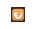
\includegraphics{include/icn_firefox.png}
		\label{fig:iconefirefox}
		\caption{L'icône du navigateur Mozila Firefox}
	\end{figure}\par

\section{Utiliser le moteur de recherche Lilo}

\chapter{Mises à jour}
	\subsection{Pourquoi faire les mises à jour ?}
	\subsection{Effectuer les mises à jour}

\chapter{Bonnes pratiques}
	\section{Entretien du matériel}
	\section{Sécurité sur internet}

\chapter{Avancé}
\section{Utiliser l'invit de commande}\label{sec:utiliserterminal}
	\subsection{Présentation de l'invit de commande}
	\subsection{Les commandes de bases}


\end{document}